\newpage
\section{Background}
\label{chapter:background}
% max 10 pages

\subsection{Modelling Framework}

\subsubsection{Structural Causal Model}
Throughout this thesis we will assume that the data is generated by a Structural Causal Model (SCM) $\C{M}$. This modelling framework is widely used in the field of causality, and is very flexible (see e.g. \citet{pearl2009causality} and \citet{peters2017elements} for the variety of methods). 

A distinction is made between endogenous variables and exogenous variables. Endogenous variables are known, either by measurement (data $\B{X}$) or by design of some inference method (e.g. context variables $\B{C}$ in LCD). They are represented by an index set $\C{I}$. Exogenous variables are latent, a typical example is noise variables $\B{N}$. Exogenous variables are represented by an index set $\C{J}$.

The causal mechanism $\B{f}$ of a SCM is a function that describes how all variables relate to each other. It maps a product space of all variables to a product space of the endogenous variables. 

The components of the causal mechanism $f_i$ usually do not depend on all variables, but rather on a small subset that we call the parents $\pasub{}{i}$ of variable $X_i$. The augmented graph $\C{H}_{\C{M}}$ represents these child-parent relations with directed edges between variable nodes.

The exogenous variables are modelled with a product probability measure $\Prb_{\BC{E}}$, since their values are not measured. Data can then be sampled from a SCM by sampling from this measure and (iteratively) applying the functions $f_i$ to compute the values of the endogenous variables.

Usually, an incomplete definition of SCMs suffices, consisting of the structural equations of the endogenous variables and the density function of the exogenous variables, indicated below with $\B{X}$ and $\B{E}$ respectively:

$$\C{M}: \begin{cases}
    X_i &= f_i(\B{X}_{\pasub{}{i} \cap \C{I}}, \B{E}_{\pasub{}{i} \cap \C{J}}) \\
    p_{\B{E}} & = \prod_{j\in\C{J}} p_{E_j}
\end{cases}$$

In a practical setting we are unable to infer the real structure of the exogenous variables. A useful graphical representation of a SCM is the graph $\C{G}_{\C{M}}$, which is an abstraction of the augmented graph $\C{H}_{\C{M}}$. Only the endogenous variables are nodes in this graph. The relations among endogenous variables are still represented by directed edges ($i \to j$). Variables that are confounded by an exogenous variable (i.e. share an exogenous ancestor) are connected with a bidirected edge\footnote{The same representation of confounding is used when we marginalize over a subset of endogenous variables.} ($i\oto j$).

\subsubsection{Causal Assumptions and Interventional Data}
If one observes two variables $X$ and $Y$, and measures a dependence among them, it is impossible to say if $X$ causes $Y$ or the other way around. More formally, one cannot infer the causal direction from a probability measure $\Prb_{\{X,Y\}}$ alone. This is why we have to rely on \textit{causal assumptions} \citep{pearl2009causality}. Some common assumptions are discussed in Section \ref{sec:back:prin}. Section \ref{sec:back:meth} describes inference methods that rely on these assumptions. 

One assumption particularly relevant to this thesis is related to the method of data acquisition. A distinction is made between \textit{observational data} and \textit{interventional data}. Observational data is gathered without interference with the system. We assume that there is an underlying SCM, and every data point is a sample from it. The sampling distribution approximates the observational distribution $\Prb_{\B{X}}$. It is theoretically impossible to infer any causal statements without further assumptions. 

Interventional data is gathered while we interfere with the system. Every data point is measured while an \textit{intervention} is performed. Formally, this intervention is modelled as a manipulation of the causal mechanism $\B{f}$ subject to some constraints or assumptions. This may render the causal inference problem theoretically possible. 

A concrete example is the \textit{perfect intervention}. A perfect intervention sets a variable $X_i$ to a fixed value $\xi_i$, denoted as $\intervene(X_i=\xi_i)$. This removes all the dependence of $X_i$ on its parents $\pasub{\C{H}}{i}$. The adapted SCM induces a different, interventional distribution $\Prb_{\B{X}|\intervene(X_i=\xi_i)}$. \citet{pearl2009causality} developed a do-calculus that can be used to make causal inferences from observational and intervenional data. As a simple example, take a system of two variables that are related as $X\to Y$. From the observational data we only know that $X$ and $Y$ are dependent. However, if we have access to distributions $\Prb_{\{X,Y\}|\intervene(X=x)}$ and $\Prb_{\{X,Y\}|\intervene(Y=y)}$ we can see that intervening on $Y$ does not affect $X$, whereas intervening on $X$ does affect $Y$. We conclude that $X$ causes $Y$. 


\subsubsection{Markov Property}
The Markov Property is a very common assumption that links the SCM to conditional independence relations (CIRs) in the data. The property follows from the definition of the SCM, so it does not add a restriction to our modelling. 

The notion of \textit{d-separation} is used to infer CIRs. We say that two variables $X$ and $Y$ are d-separated by a conditioning set of variables $\B{C}$, if all walks in $\C{G}_{\C{M}}$ from $X$ to $Y$ are d-blocked by $\B{C}$. This is denoted as $\dsep{X}{Y}{\B{C}}{\C{G}}$. On each walk we will consider if the variables are a \textit{collider}, that is: if the adjacent edges of the walk point towards it ($...\to Z \ot ...$). A walk is \textit{d-blocked} in three cases:

\begin{compactenum}
    \item $X$ or $Y$ are in $\B{C}$.
    \item The walk contains a non-collider $Z$ that is in $\B{C}$.
    \item The walk contains a collider $Z$ that is not in $\B{C}$, and none of its descendents are in $\B{C}$ either.
\end{compactenum}

Consider the graph in Figure \ref{fig:2:dsep}. By case 1, $X_1$ blocks the walk from $X_1$ to $X_3$. $X_2$ blocks this walk if it is in the conditioning set $\B{C}$ by case 2. According to case 3, the walk from $X_2$ to $X_4$ is blocked if neither $X_3$ nor $X_5$ are in $\B{C}$.

\begin{figure}[h]
    \centering
    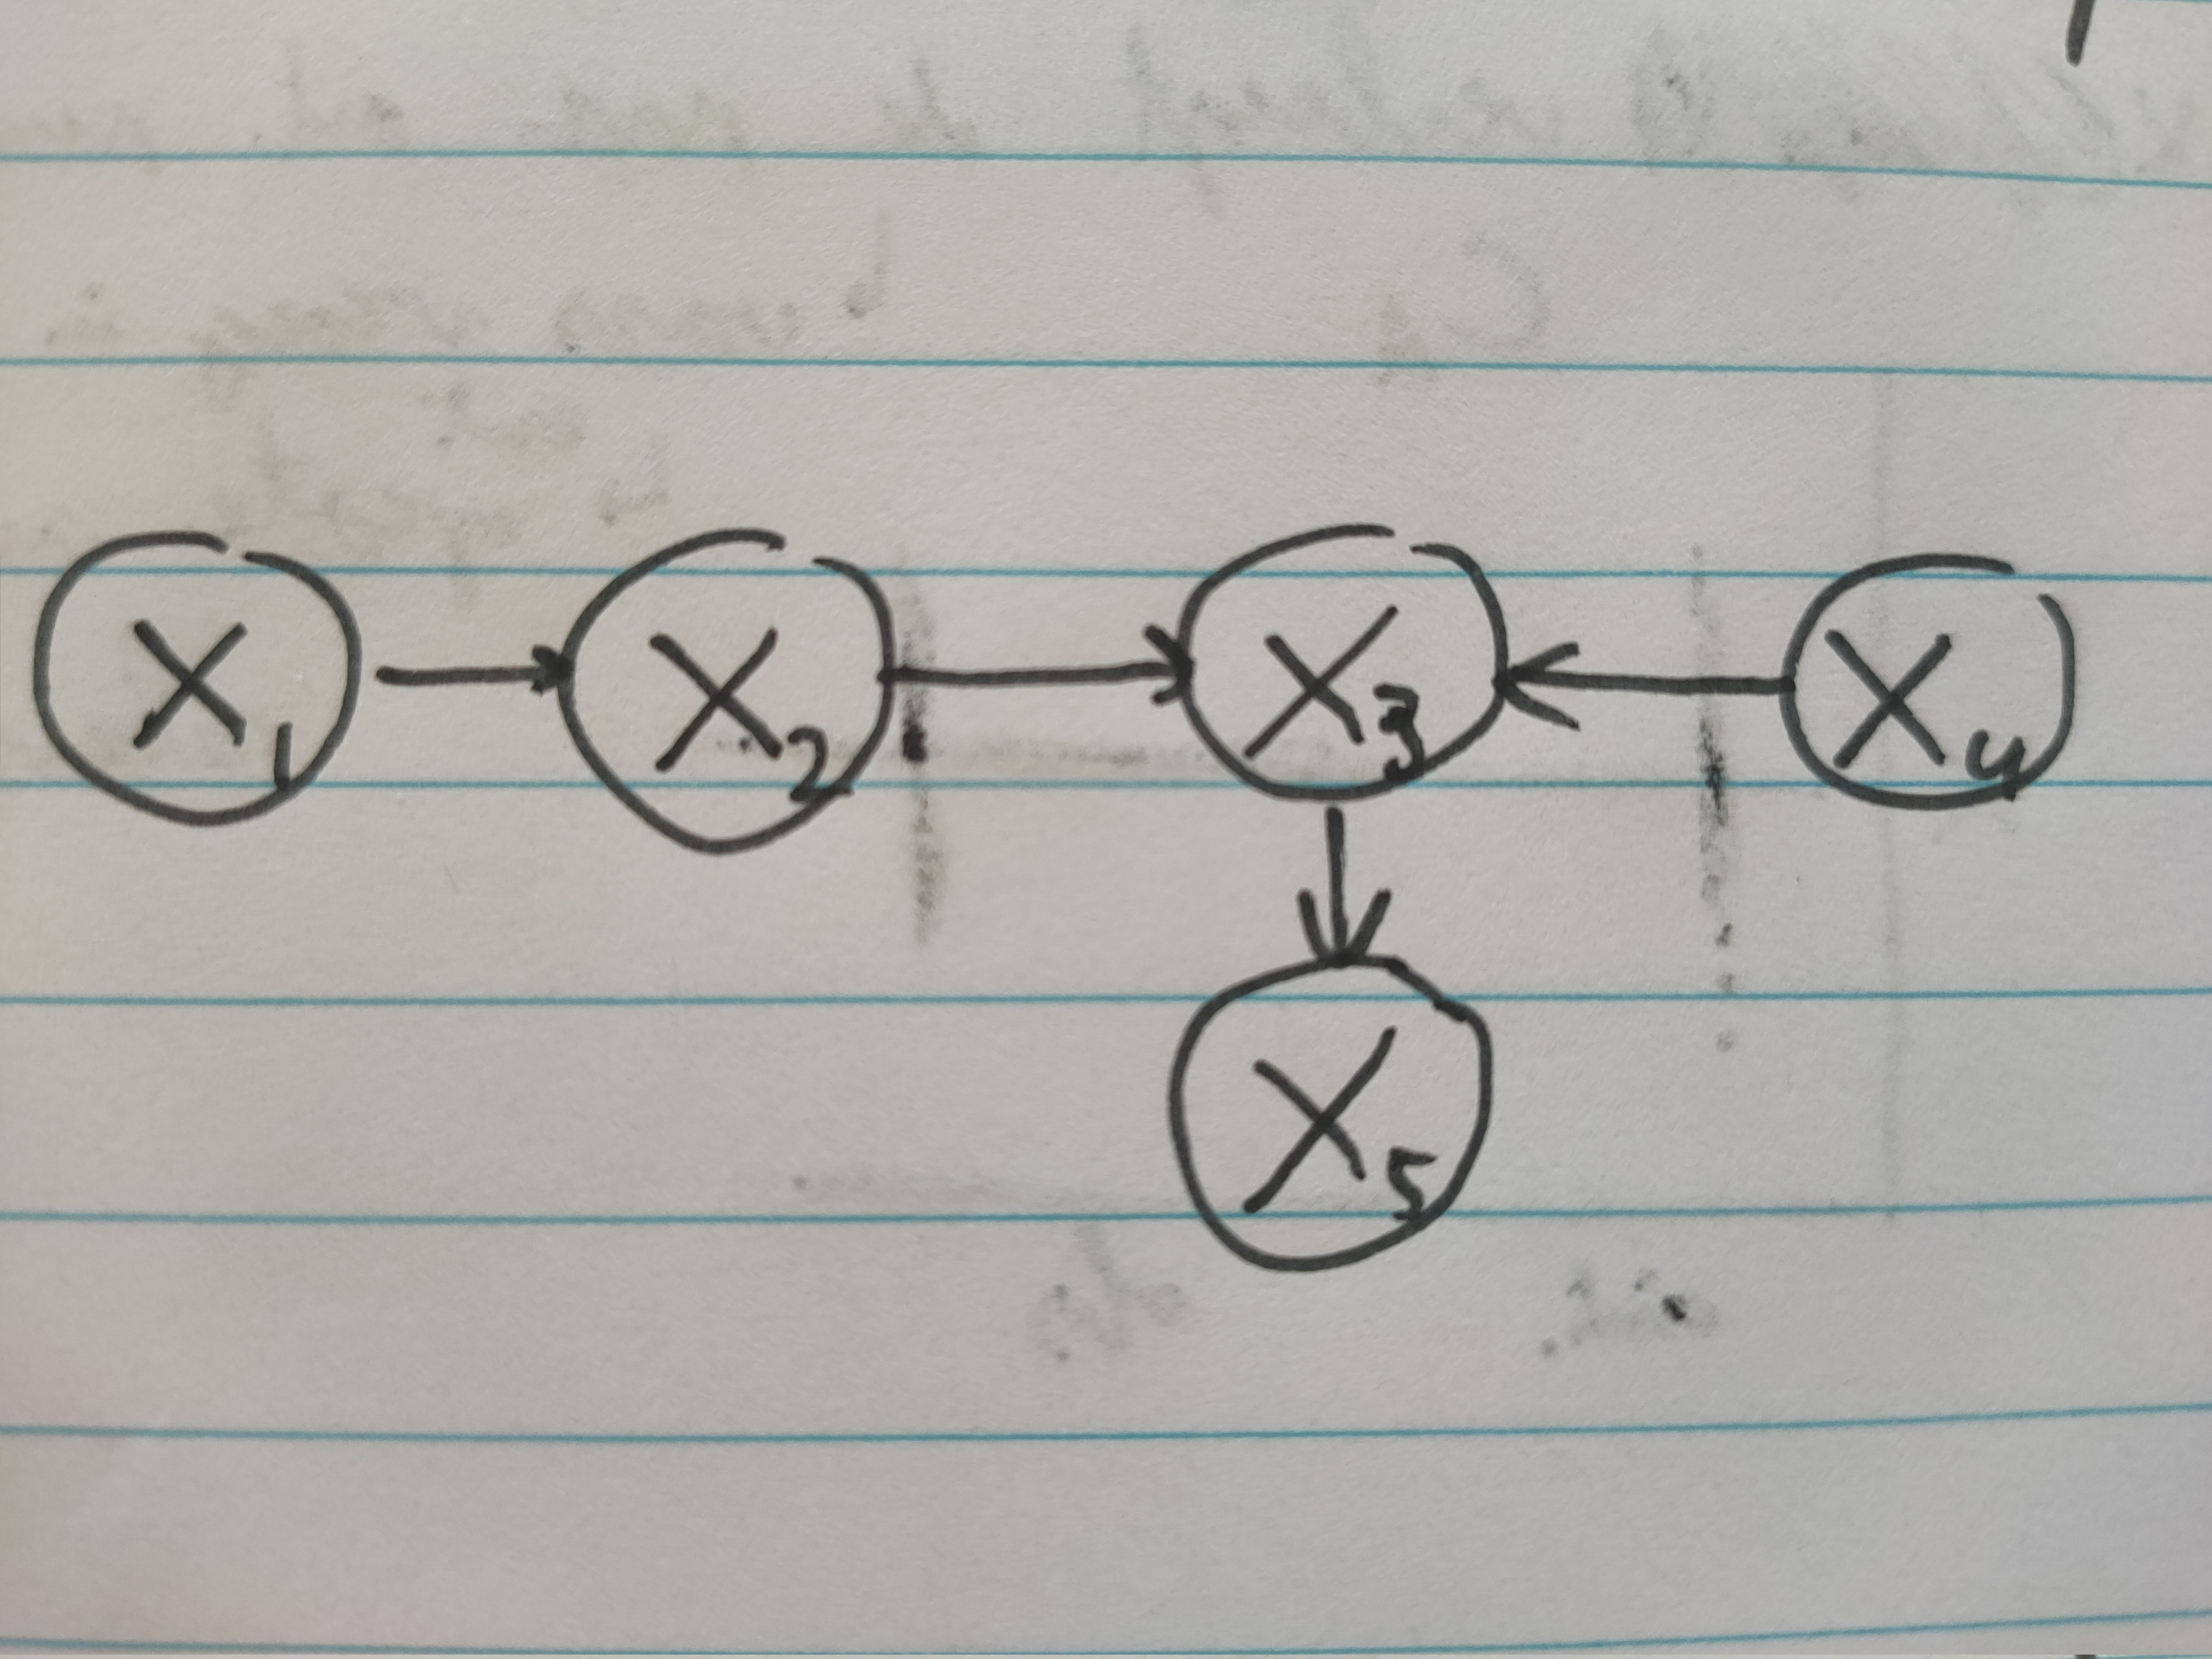
\includegraphics[width=\textwidth]{2dsep}
    \caption{Graph of five random variables.}
    \label{fig:2:dsep}
\end{figure}

The Global Markov Property links d-separation to conditional independence:

$$\dsep{\B{A}}{\B{B}}{\B{C}}{\C{G}} \implies \indep{\B{A}}{\B{B}}{\B{C}}{\Prb_{\B{X}}}$$

The Markov Property with d-separation is only valid for SCMs with an acyclic graph.\footnote{It is also valid for some restricted cases of cyclic SCMs, cf. \citet{forre2017markov}.} A generalization of d-separation was developed by \citet{forre2017markov} that applies to the cyclic case as well under certain assumptions.

Different graphs may satisfy the same set of d-separations. Therefore, some observational distribution $\Prb_{\B{X}}$ may satisfy the Global Markov Property with respect to different graphs. The set of graphs that induces the same observational distribution as some graph $\C{G}$ is called its Markov Equivalence Class $\mec(\C{G})$. For acyclic graphs without latent confounding, it is shown that two graphs are equivalent if they have the same skeleton and immoralities \citep{verma1991equivalence}. The skeleton is the set of edges when we disregard their direction, an immorality is a local structure $A\to B \ot C$ in which $A$ and $C$ are not directly connected.
% \footnote{Formally, one graph may induce multiple distributions, and the MEC consists of graphs that induce the same distributions.}

Causal inference methods that use only CIRs in observational data cannot infer more than the MEC of the graph, because this is all the information that is in the CIRs in the observational distribution $\Prb_{\B{X}}$.


\subsubsection{Causal Inference Tasks}
Different tasks can be distinguished within causal inference. In this thesis we focus on methods that infer parts of the augmented graph $\C{H}$. These methods are not directly used to infer quantitative causal effects. However, the do-calculus of \citet{pearl2009causality} can in many cases be used to combine measured conditional distributions and a (partially) infered graph to make quantitative statements.

Generally, we can distinguish between global and local inference methods. Global methods aim to infer as much as possible from graph $\C{G}$. If the data is observational, these methods infer (an instance of) the MEC. An example is the SGS algorithm \citep{spirtes2000causation}, which naively checks the CIRs among all combinations of variables to infer the MEC. Interventional data enables some methods to infer more features of the graph, like Greedy Interventional Equivalence Search by \citet{hauser2012characterization} that infers a so-called interventional MEC. 

Local methods are specialized to find only some elements of the graph, usually trading completeness for efficiency. Commonly, these methods find some direct or ancestral causal relations (directed paths in $\C{G}$), like Local Causal Discovery \citep{cooper1997simple} which tests for one specific pattern of CIRs among three variables.


\subsection{Principles of Causal Inference}
\label{sec:back:prin}

\begin{figure}[h]
    \centering
    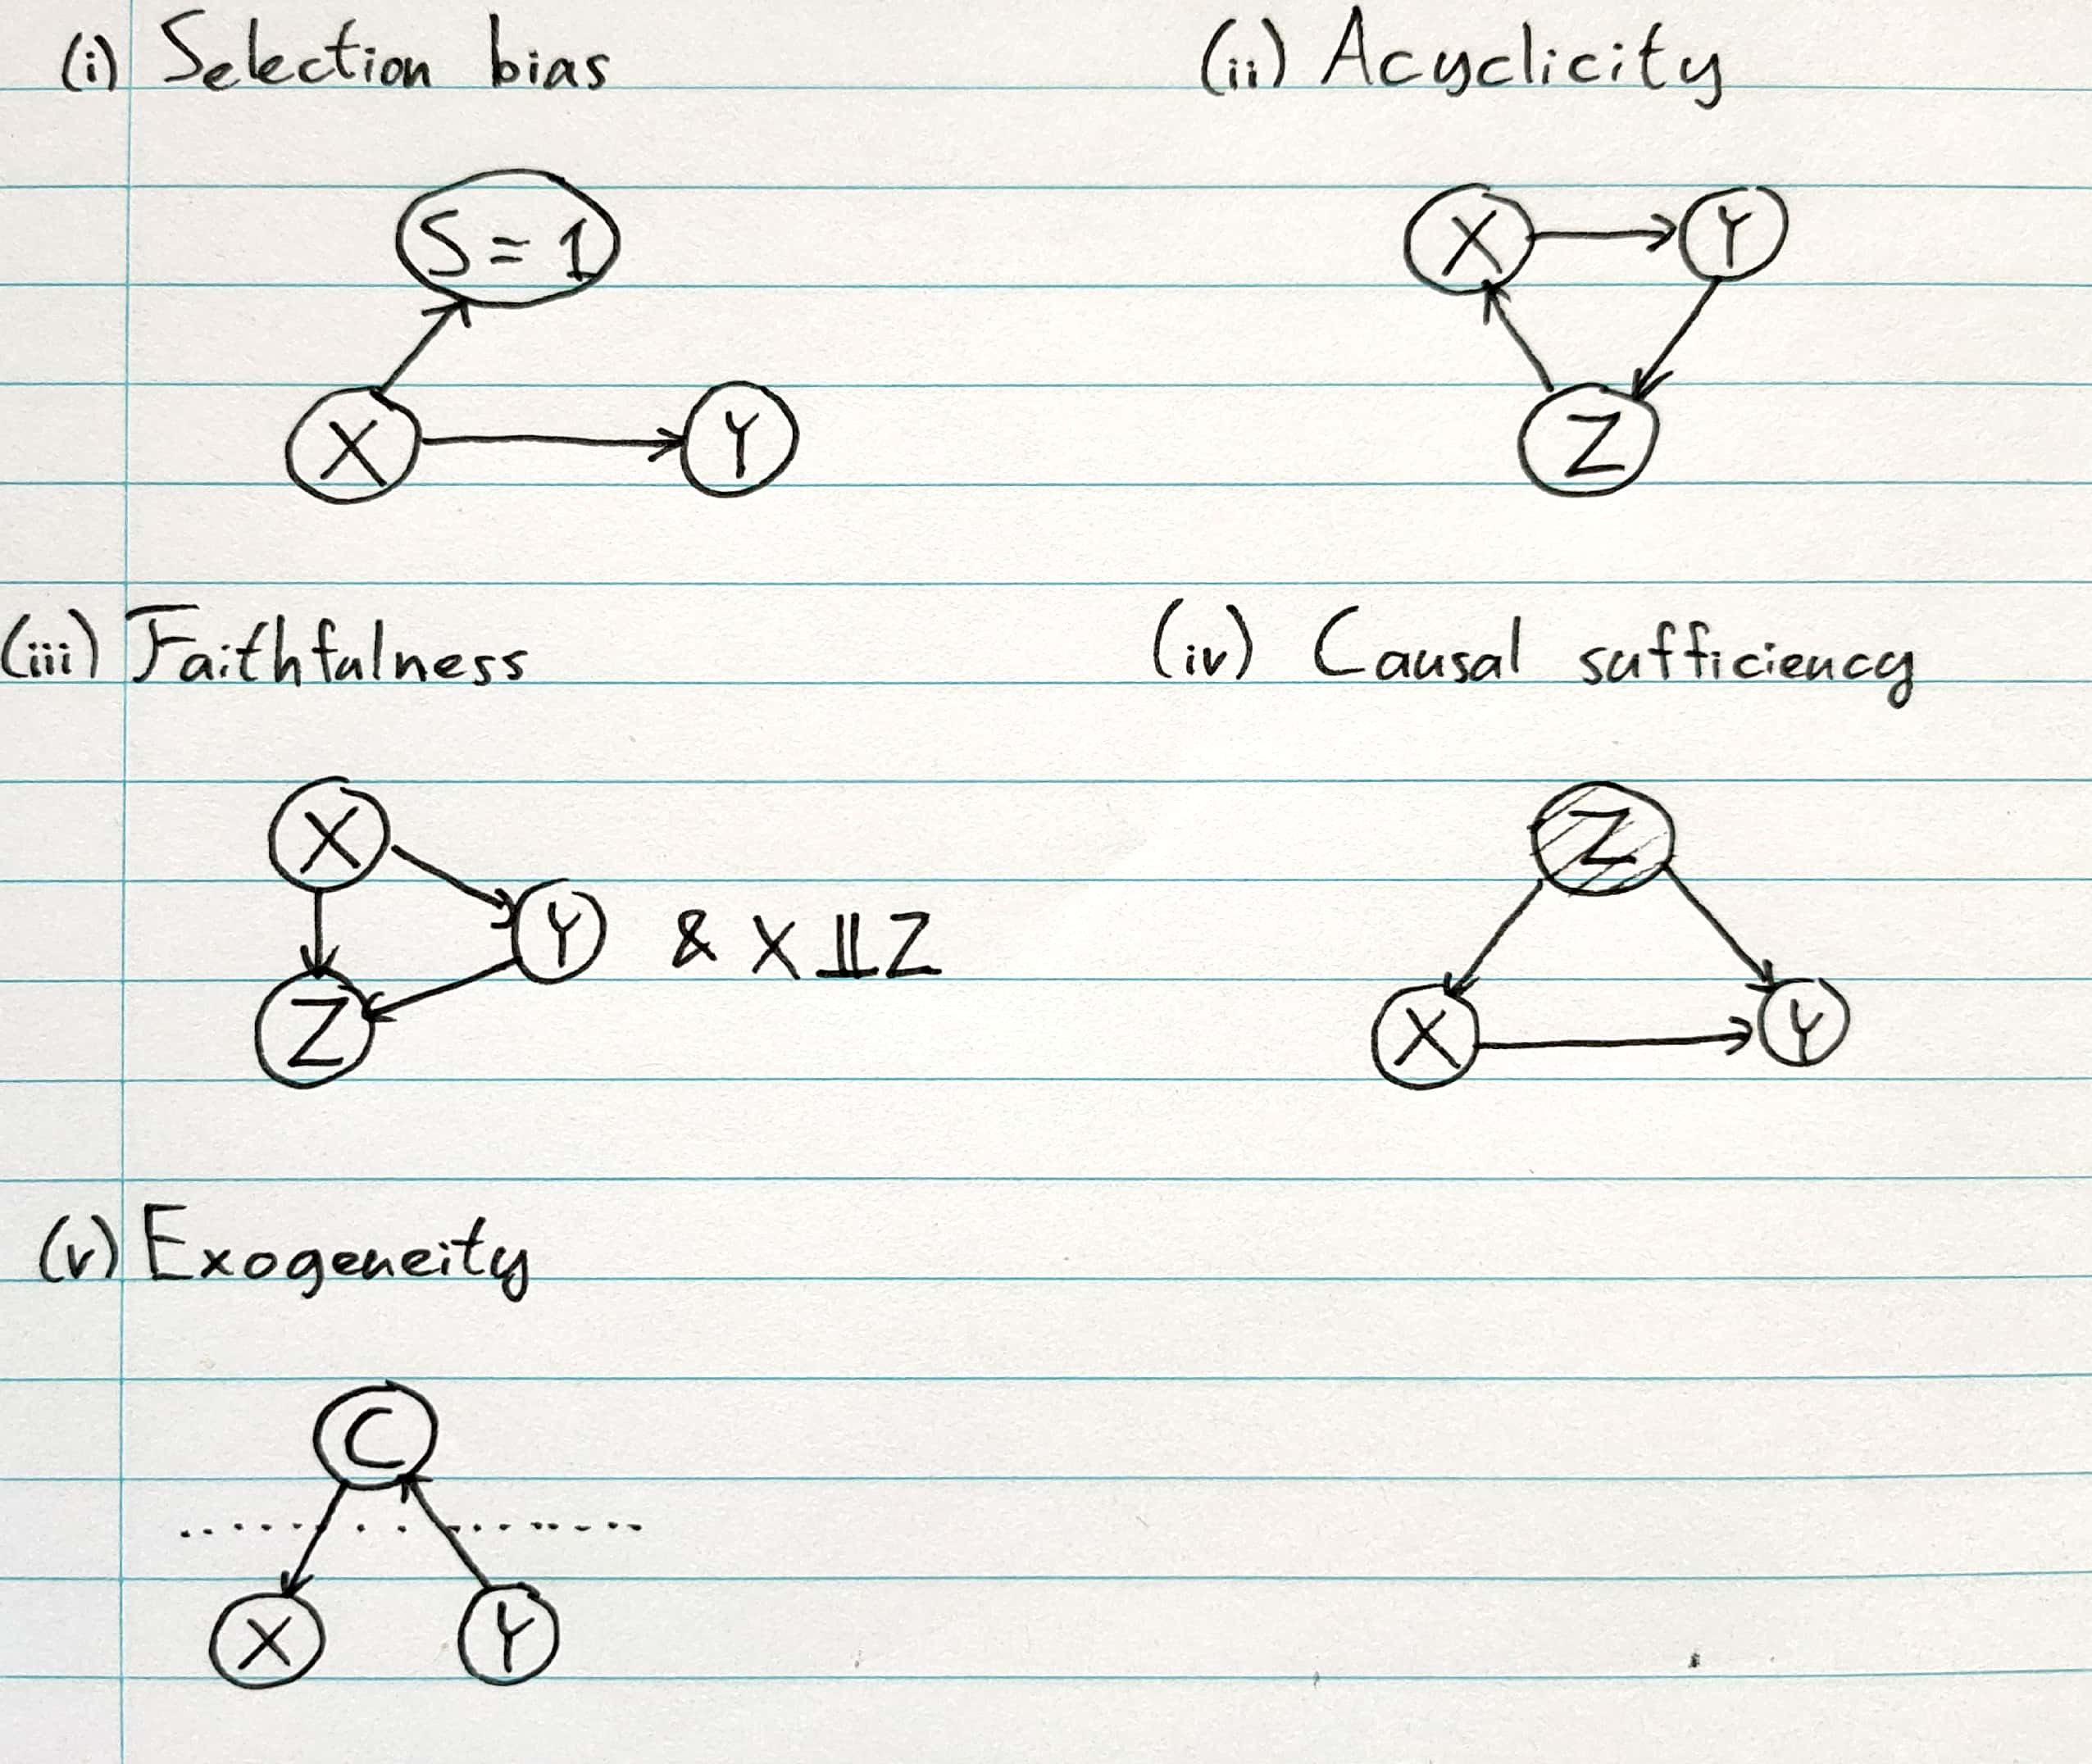
\includegraphics[width=\textwidth]{2assumptions}
    \caption{Violations of causal assumptions indicated by orange nodes or edges. Violation of faithfulness (iii) depends on the functional dependence between the variables, for example if $X \CI Z$.}
    \label{fig:2:ass}
\end{figure}

Now that the general modelling framework of the SCM is established, it is time to define the most important additional assumptions that enable many causal inference methods. These assumptions are generally restrictions on the SCM.

\subsubsection{Reichenbach's common cause principle}

An important insight in causal inference is Reichenbach's common cause principle \citep{reichenbach1956direction}. It states that correlation is always the result of some causation. When two variables correlate, either one causes the other, or there is a third variable causing both. 

This is quite a strong assumption. It relies on i.i.d. sampling of the data, and a good approximation of the probability distribution. One should be cautious for spurious correlations. These can result from a search over correlations between many variables (without type I error control), or from overseeing a time dependence of the variables (violation of i.i.d. assumption). 

Moreover, the principle relies on the important assumption of \textbf{unbiased data selection}. Selection bias can be present when data selection is based on the value of some unobserved variable that is the effect of some observed variables. Take for example the graph in Figure \ref{fig:2:ass}i. Suppose that $X$ and $Y$ happen to correlate in the specific case that $S=1$, an example of a spurious correlation. If we only have data with this value of $S$, we could erroneously infer a causal relation between $X$ and $Y$.

This assumption is required for many causal inference methods. Take for example Local Causal Discovery (LCD) \citep{cooper1997simple}, which depends on some local pattern of CIRs to infer an ancestral relation. If CIRs can be the result of selection bias, the pattern is not sufficient anymore to infer the ancestral relation.


\subsubsection{Faithfulness}

\textbf{Faithfulness} is a very common assumption. It reverses the implication of the Markov Property, such that conditional independence implies d-separation in the graph:

$$\indep{\B{A}}{\B{B}}{\B{C}}{\Prb_{\B{X}}} \implies \dsep{\B{A}}{\B{B}}{\B{C}}{\C{G}}$$

Many causal inference methods use this assumption to restrict the set of possible graphs by measuring conditional dependences and independences. The test used to measure dependences and independences relies on additional assumptions, which we jointly call the assumption of a \textbf{perfect independence test}. For example, the partial correlation test relies on normality of the data. When the data and assumptions are sufficient to infer the MEC of the graph, we say that the MEC is \textbf{identifiable}.

Faithfulness may be violated. Take the graph in Figure \ref{fig:2:ass}iii. Some causal mechanism may result in an independence between $X$ and $Z$, even though $Z$ is functionally dependent on $X$ and an intervention on $Y$ would show this.

It may be problematic that faithfulness requires that all CIRs in the data are in the graph. Especially when the graph is large and contains cycles, there may be hypothesis testing errors \citep{uhler2013geometry}.

% \silvan{ADD: Conditional independence testing has been proven to be impossible when no additional assumptions are imposed on the distributions involved (Shah and Peters, 2019) [P. Boeken]}

An implication of faithfulness is \textbf{causal minimality}. A distribution satisfies causal minimality with respect to some graph if it is Markov to the graph, but not to any proper subgraph. 

One method that relies on faithfulness is Accounting for Strong Dependences (ASD) \citep{hyttinen2014constraint}. All dependence and independence relations are encoded as soft constraints in an Answer Set Programming (ASP) solver, along with constraints that determine how CIRs relate to the graph structure.

\subsubsection{Causal sufficiency}

The presence of latent (unobserved) variables can make it harder to identify parts of SCMs. Latent confounders that affect multiple variables influence the CIRs. Some methods rely on the \textbf{causal sufficiency} assumption that there are no latent confounders. Figure \ref{fig:2:ass}iv shows a violation of this assumption, where $Z$ is latent.

Inductive Causation (IC) \citep{verma1991equivalence} checks for every pair of variables $X$ and $Y$ that are dependent if there is a set of variables $\B{S}$ that renders them conditionally independent: $\indep{X}{Y}{\B{S}}{}$. If no such set exists, there must be a direct causal relation, because by Reichenbach's principle and causal sufficiency there cannot be another way in which they are dependent.

\subsubsection{Acyclicity}

The \textbf{acyclicity} assumption restricts the class of graphs to directed mixed graphs\footnote{DMGs are like DAGs, with bidirected edges that indicate latent confounding.} (DMGs). Inference under this assumption is typically easier, because the class of possible graphs is much smaller. Nevertheless, some methods can be generalized when the concept of $\sigma$-separation is introduced to replace d-separation (e.g. \citet{mooij2016joint}). 

One advantage of assuming acyclicity is that it is possible to define some ordering in the variables. In this order, variables precede their descendents in the graph. Greedy Equivalence Search (GES) \citep{chickering2002optimal} is an example of a method that exploits this property. The search for the MEC is transformed to a search for an order that corresponds to the MEC. A greedy search algorithm is used to move between permutations of the order to efficiently find the correct MEC. 

\subsubsection{Exogeneity}

Some methods distinguish between two types of endogenous variables: the system variables $\B{X}$ and the context variables $\B{C}$. The context is seen as external to the system. This means that according to the \textbf{exogeneity}\footnote{Note that 'exogenous' might refer to observed, endogenous context variables, or unobserved exogenous variables as represented by $\C{H}$} assumption, no edges in the graph can point from a system variable to a context variable. 

This assumption is violated in the graph in Figure \ref{fig:2:ass}v. We observe an effect on $X$ when we intervene on $Y$. If we assume that $C$ is exogenous, we could erroneously conclude that there is a direct relation $Y\to X$. In this case however, $C$ mediates this relation.

Typically, the context variables are used by the modeller to encode some causal background knowledge, such as the type of intervention. Invariant Causal Prediction (ICP) \citep{peters2016causal} leverages the exogeneity assumption to compare the conditional distribution of a variable given a set of potential parents, across values of the context. If the context itself is not a direct parent of the variable, this conditional distribution should be invariant, which allows ICP to infer causal relations. 

\subsection{Causal Discovery Methods}


\subsubsection{Constraint-Based Causal Discovery}
Constraint-based approaches derive constraints from the data, and use it to restrict the class of possible underlying causal graphs. Causal inference is treated as a constraint-satisfaction problem. Generally, conditional independence relations (CIR) are chosen as constraints, which can be used to derive the separation of variables and the orientation of edges in the graph. Some prominent methods are described below.

\textbf{Inductive Causation} (IC) was introduced by \citet{verma1991equivalence} and generally describes how we can induce a PDAG from conditional independences in the data. The algorithm consists of two steps: inducing the skeleton and orienting the edges. For every pair of variables $a$ and $b$, we check whether there is an edge in the PDAG. Using the faithfulness assumption, we add an edge if there is no separating set of variables $S_{ab}$ that makes $a$ and $b$ conditionally independent ($\nexists S : \indep{a}{b}{S_{ab}}{}$). One easy step of edge orientation uses the separation criterion of colliders. If two non-adjacent variables $a$ and $b$ share a neighbour $c$ that is not in $S_{ab}$, it must be a collider on the path and we induce edge orientation $a\to c \ot b$. Application of additional orientation rules lead us to a maximally oriented PDAG, which describes the Markov equivalence class of all causal graphs that induce the joint data distribution. One early set of such rules was described by \citet{spirtes2000causation} in the SGS algorithm, which was named after the authors.
            
IC is quite limited, because it relies on several assumptions about the underlying SCM (e.g. causal sufficiency), and its naive implementation is costly due to the search over all separating sets $S_{ab}$.

\textbf{PC}, named after its inventers Peter Spirtes and Clark Glymour \citep{spirtes1991algorithm}, reduces the cost of naive IC. A systematic algorithm finds the separating sets $S_{ab}$ in polynomial time. Starting from a fully-connected graph, edges are systematically removed by considering separating sets of increasing cardinality, and only taking into account the variables that neighbour $a$ and $b$. For example, first edges are removed between variable pairs that are independent given the empty set (cardinality 0). Then, edges are removed between remaining adjacent variable pairs that are independent given one of their neighbours. Already some possible separating sets can be skipped here, because edges were removed in the previous step. Therefore, as we consider larger possible separating sets, the number of neighbours to choose from decreases.
            
\textbf{Fast Causal Inference} (FCI) extends PC to allow for selection bias and latent confounding. Dropping the causal sufficiency assumption, means that it should consider some possible separating sets $S_{ab}$ that contain variables not adjacent to $a$ or $b$ (specifically, their ancestors). FCI is a feasible algorithm for datasets with many variables when the underlying graph is sparse and bidirected edges are not too much chained together. It was first introduced by \citet{spirtes1999algorithm}, and gradually developed since then. A modern version named FCI+ by \citet{claassen2013learning} is relatively fast. It finds the complete PAG in polynomial time.
            
\textbf{Invariant Causal Prediction} (ICP) does not infer a complete equivalence class of causal graphs from the data, but is concerned with local features of that graph. In its original formulation by \citet{peters2016causal} it outputs a subset of parents of a target variable, and in a later adaptation by \citet{mooij2016joint} the output is a subset of ancestors. In comparison to the previous methods, this approach uses data from different contexts.

When we model the context (e.g. intervention) as a variable that is not a cause of the target variable, then the conditional distribution of the target variable given its direct causes is invariant to the value of the context variable. This property is used by ICP to find parent or ancestor relations in data from different contexts. 

In a naive implementation, we would have to investigate every possible parent set for every target variable, making the complexity exponential in the number of variables. Since (direct) causes tend to correlate with their effect, it is reasonable to only consider variables that have a relatively high correlation with the target variable. Such an approximation was used by \citet{peters2016causal} and \citet{meinshausen2016methods} to apply ICP to the dataset of \citet{kemmeren2014large} with over six thousand variables.

\textbf{Local Causal Discovery} (LCD) is a simple local method that looks at ancestral causal relations in the context of a changing environment. In the data, we marginalize over three variables ($C, X, Y$), one of which is exogenous ($C$). This means that we have the domain knowledge that this variable is not a direct or indirect effect of any endogenous variables. Next, we perform three statistical tests: $\indep{C}{Y}{X}{}$, $C \nCI X$ and $X \nCI Y$. If these tests are positive, \citep{cooper1997simple} proves that there is a relationship $X \to Y$. 

This method allows for latent confounders, and assumes that there is no selection bias. Note that this method can find only a limited subset of ancestral relations. \citep{cooper1997simple} prove the theory by listing all possible causal graphs of three variables in which the context variable is not caused by endogenous variables. They note that of the 32 networks in which $X$ causes $Y$, LCD is only able to identify this relation in 3 cases. The others are not identified, because there are other configurations that induce the same independence relations. For example, if $C$ causes $Y$ not only through $X$, but via another path as well, we will not find that $X$ causes $Y$.  

% e.g. Trigger?\citep{chen2007harnessing}. Local strategy.

\textbf{Y-structures} are a pattern in a Partial Ancestral Graph (PAG), which has information about ancestral relations between four random variables. \citet{mooij2015empirical} showed that a set of independence tests can be used to infer some ancestral relations from observational data. This local method can be used to find an incomplete set of ancestral relations in the underlying SCM. 

Specifically, we marginalize over four random variables $X$, $Y$, $Z$ and $U$. Then we perform four statistical tests: $\indep{Z}{Y}{X}{}$, $Z \nCI Y$, $\dep{Z}{U}{X}{}$ and $Z \CI U$. If all tests are positive, there are only two possible PAGs representing the marginalization over the four variables, which are called Y-structure (a term coined for a score-based method by \citet{mani2006bayesian}) and Extended Y-structure. In both PAGs, we can use the backdoor criterion to infer that $p(Y\given \intervene(X=x))=p(Y\given X)$.

\citet{mooij2015empirical} investigate the performance effect of adding more independence tests. By adding two more tests, the Y-structure remains the only possible PAG. After that, more redundant independence tests can be added. Adding more tests necessarily reduces recall, but precision can improve if the extra tests eliminate false positives. Interestingly, in their experiments on synthetic data, maximum precision is not always achieved with the minimum or maximum number of tests.

An interesting insight from \citet{mooij2015empirical} is that the faithfulness assumption becomes more problematic as the number of random variables grows. The data is sampled from a SCM, which makes the faithfulness assumption very reasonable. However, it appears that the marginalized data can be almost faithless to the supposed PAG. 

% Mooij2015empirical: Our  findings  illustrate  that  violations of strong faithfulness become increasinglylikely  in  the  presence  of  many  latent  variables,and  this  can  significantly  deterioriate  the  accu-racy of constraint-based causal prediction algo-rithms that assume faithfulness.


    
\subsubsection{Score-Based Causal Discovery}
Score-based approaches search for the causal graph that optimizes some loss function, often based on independences in the data. Some methods are discussed below.
% (e.g., Cooper and Herskovits,1992; Heckerman et al., 1995; Chickering, 2002; Koivisto and Sood, 2004) (see: Peters 7.2)
% Mani et al 2006: disadvantages of constraint-based (citing Heckerman et al., 1999): (1) the inability to include prior belief in the form of structure probabilities, (2) the output is based on the significance level used for the independence tests, and (3) there is no quantification of the strength of the hypothesis that is output.

\textbf{Accounting for Strong Dependences} (ASD) is a method that focusses on graphs satisfying dependences in the data, whereas most methods focus on the independences. The groundwork of the method was layed by \citet{hyttinen2014constraint}. Dependence and independence relations in the data are encoded as soft constraints in ASP (Answer Set Programming), together with rules that determine that the solution should be a valid graph. The solution is then found by an ASP solver, that minimizes the loss computed as the sum of the weights of the constraints that are not satisfied. This method can only be applied to problems with a small number of variables, because the number of dependence and independence relations quickly becomes very large.

\citet{magliacane2016ancestral} compute weights based on the p-value of the conditional independence test and the significance level, such that strong dependences obtain a larger weight than independences. They also provide a method to compute a confidence score for single features of the graph (like an ancestral relation) by solving two optimization problems and subtracting the losses. In one problem, the presence of the feature is added as a hard constraint, in the other the absence is added as a hard constraint. 

As part of their Joint Causal Inference (JCI) framework, \citet{mooij2016joint} adapt the ASD method to include interventional data. They simply add some constraints to the ASP problem that encode their JCI assumptions for interventional data.

\textbf{Greedy Equivalence Search} (GES) was first introduced by \citet{meek1997graphical} and further detailed by \citet{chickering2002optimal}. A search for the Markov equivalence class (MEC) is performed in two phases. Our graph is initialized without edges. In the first phase, we move between MECs by adding edges. In each step, we consider the set of MECs that are one edge addition away from the current MEC. Reversing a covered edge does not change the MEC, so we need to consider every combination of covered edge reversals, followed by a single edge addition, followed by covered edge reversals. We score the MECs and move to the one with the highest score. \citet{meek1997graphical} proposed the Bayesian scoring criterion to score DAGs in a MEC. Under some conditions this can be approximated by the Bayesian information criterion (BIC). 

Once we reach a local maximum, \citet{chickering2002optimal} shows that the MEC contains the generative distribution. The second phase is analogous to the first, but this time single edges are removed. \citet{chickering2002optimal} shows that this final MEC is a perfect map of the generative distribution.

\citet{hauser2012characterization} generalize the method to datasets with interventional data (GIES). They introduce the interventional MEC as the object of the search. The algorithm is adapted by introducing the turning phase. Repeated application of the three phases leads to the interventional MEC underlying the generative distribution. They note that the space of interventional MECs is more fine-grained, meaning that this type of data leads to improved identifiability.


\subsubsection{Hybrid methods}
% \textbf{Max-Min Hill-Climbing} (MMHC) (Tsamardinos et al., 2006), for example, alternates between constraint-based and score-basedupdates.

\textbf{Sparsest Permutation} (SP) is a method proposed by \citet{raskutti2018learning} that searches for the Markov equivalence class in a space of topological orderings of random variables, using observational data. The topological ordering is a permutation of variables in which ancestors precede descendents. Given an ordering and a method to infer dependence and independence relations, we can infer a DAG that satisfies causal minimality. The SP algorithm searches over these DAGs infered from all possible permutations and selects the DAG with the smallest number of edges. \citet{raskutti2018learning} show that this algorithm is consistent, which means that it finds a DAG in the correct Markov equivalence class. This consistency relies on an assumption that is weaker than faithfulness. 

\citet{solus2017consistency} propose a greedy algorithm (GSP) that increases the number of variables that can be handled from about 10 to hundreds. The only sacrifice is that a somewhat stronger assumption is required, which is still weaker than faithfulness. They introduce the DAG associahedron, a sub-polytope of the permutohedron which indicates possible directions for the depth-first search \silvan{Is it a DFS or a BFS for the first MEC that is sparser, than a greedy step?}. These directions are based on the concept of covered edge. 

\citet{wang2017permutation} adapt the algorithm further to take interventional data into account (IGSP). The score is now summed over a score for each intervention distribution. This score is a weighted sum of the number of edges in the inferred graph, excluding edges into the intervened variable, and some maximum likelihood score of the interventional data given some model assumptions.



% first with consistency proof. (permutation-based without proof:  (Bouckaert, 1992; Singh and Valtorta, 1993; Teyssier and Koller, 2005). )


\subsubsection{Other methods}
other statistical patterns in the joint distribution can be exploited too (e.g Mooij et al., 2016; Peters et al., 2017)

% TODO: IDA (Maathuis et al. 2010), MMHC, CV-Lasso regression?, CI?




\label{sec:back:meth}